\textbf{\underline{\large{1.4: Local Linearity, Euler's Method, and Approximations}}} \par

Before calculators, one of the most valuable uses of the derivative was to find approximate function values from a tangent line. Since the tangent line only shares one point on the function, y-values on the line are very close to y-values on the function. This idea is called local linearity—near the point of tangency, the function curve appears to be a line. This can be easily demonstrated with the graphing calculator by zooming in on the point of tangency. \par 

Consider the graphs of $y = \dfrac{1}{4}x^4$ and its tangent line at $x = 1$, given by the equation $y = x - \dfrac{3}{4}$: \par

\begin{center}
    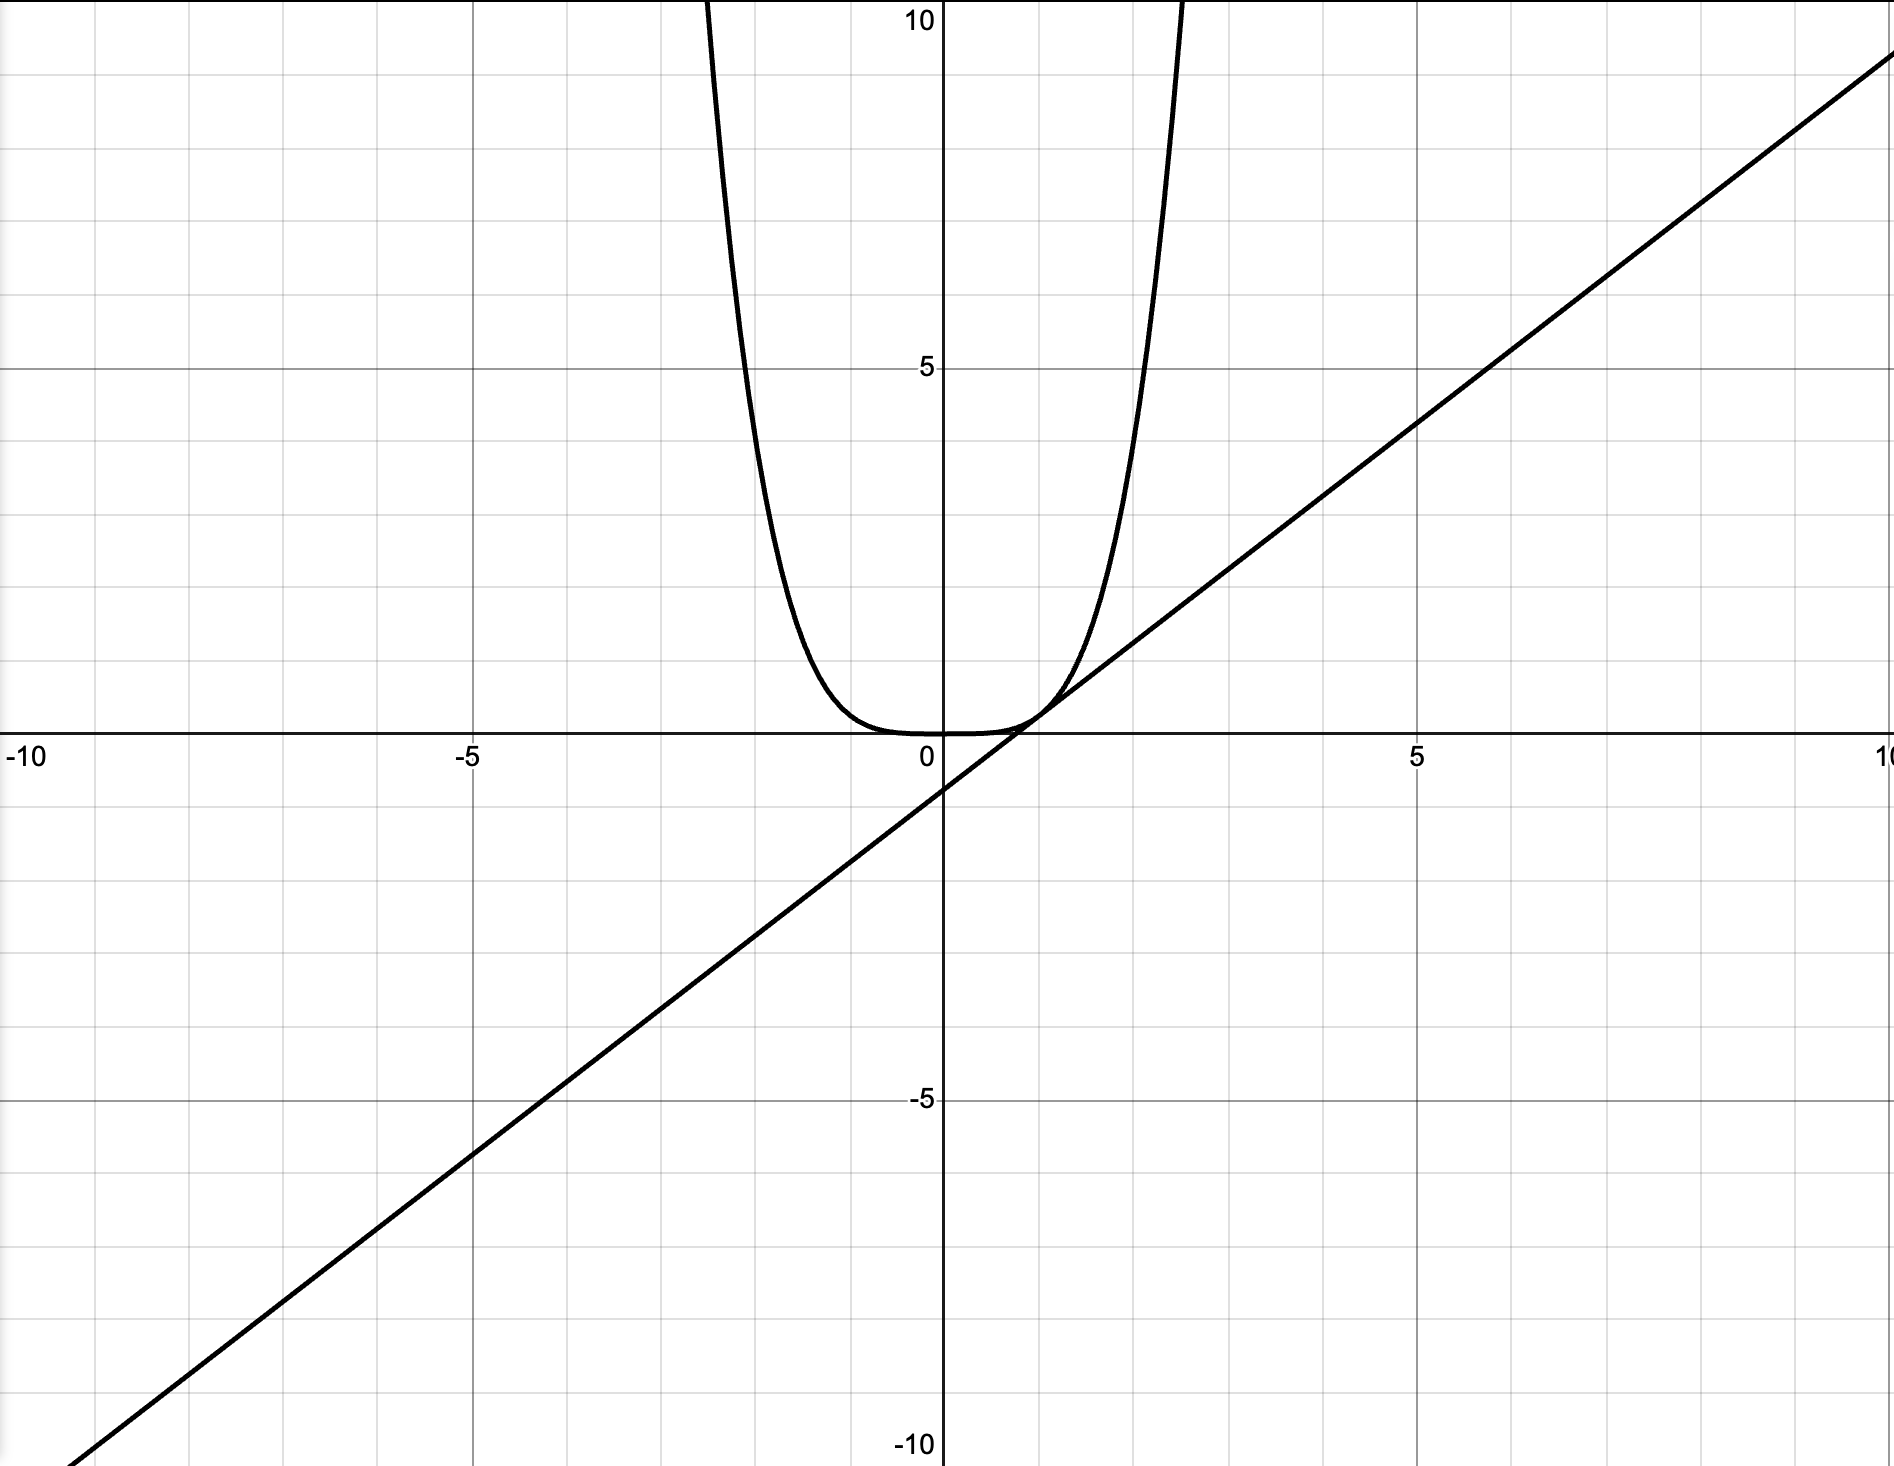
\includegraphics[width=0.49\textwidth]{Support/Chapter 1 Graphics/1.4-Graphic1.png}
    \hfill
    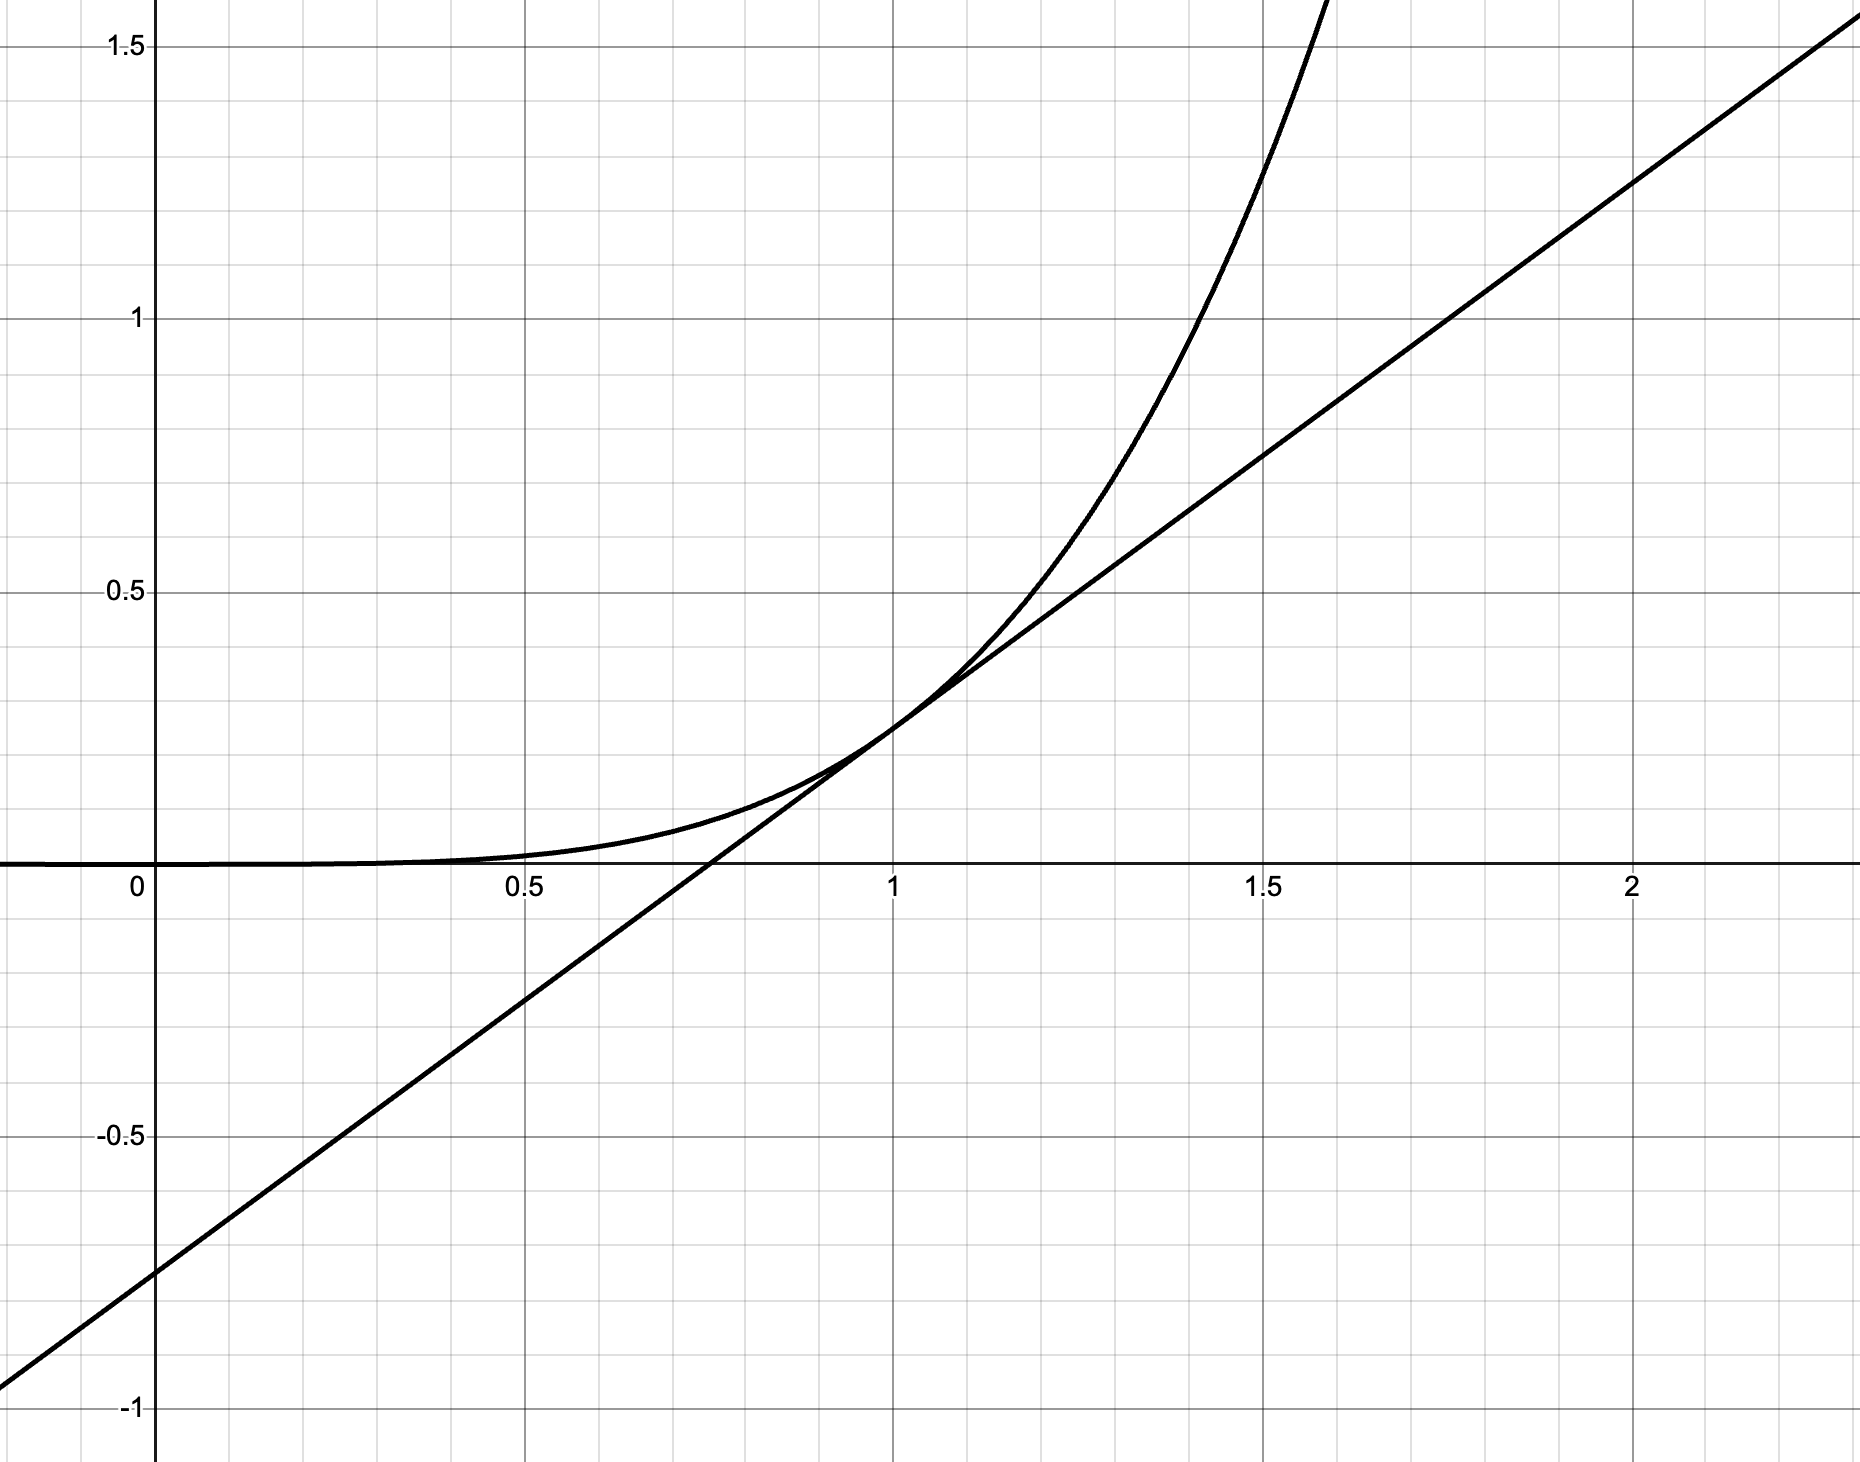
\includegraphics[width=0.49\textwidth]{Support/Chapter 1 Graphics/1.4-Graphic2.png}
\end{center}

The closer you zoom in, the more the line and the curve become one. The y-values on the line are good approximations of the y-values on the curve. For a good animation of this concept, see the following: \begin{align*}
    \href{https://drive.google.com/file/d/1lVYbRbXydqBz8KJWOfwWGO_c_oe58bC6/view?usp=sharing}{\text{\textcolor{blue}{tangent line approximation animation}}}
\end{align*} 

Since it's easier to find the y-value of a line arithmetically than for other functions --- especially transcendental functions --- the tangent line approximation is useful if you have no calculator. \par

\begin{tcolorbox}[objective]
    \begin{center}
        OBJECTIVES \\[11pt]
    \end{center}
    Use the equation of a tangent line to approximate function values.
\end{tcolorbox}

\begin{tcolorbox}[example]
    \textbf{Ex 1.4.1: } Find the equations of the lines tangent and normal to $f(x) = x^4 - x^3 - 2x^2 + 1$ at $x - 1$. 
\end{tcolorbox}
\begin{tcolorbox}[solution]
    \textbf{Sol 1.4.1: } The slope of the tangent line will be $f'(1)$ \begin{align*}
        & f'(x) = 4x^3 - 3x^2 - 4 \\[11pt]
        & f'(1) = 4(1)^3 - 3(1)^2 - 4 = -3 
    \end{align*} 
    (Note that we could've gotten this more easily with the nDeriv function on our calculator.) \begin{align*}
        & f(-1) = 1, \; \therefore \boxed{y - 1 = -3(x + 1)} \text{ or } \boxed{y = -3x - 2} 
    \end{align*} 
    The normal line is perpendicular to the tangent line and, therefore, has the negative reciprocal slope of $\dfrac{1}{3} \forcespace$.  This gives us \begin{align*}
        & \boxed{y - 1 = \dfrac{1}{3}(x + 1)}
    \end{align*} for the equation of the normal line.
\end{tcolorbox}

One of the many uses of the tangent line is based on the idea of local linearity. This means that in small areas, algebraic curves act like lines --- namely their tangent lines. Therefore, one can get an approximate y-value for points near the point of tangency by plugging x-values into the equation of the tangent line. \par

\begin{tcolorbox}[example]
    \textbf{Ex 1.4.2: } Use the tangent line equation found in \textbf{Ex 1.4.1} to get an approximate value of $f(-0.9)$. 
\end{tcolorbox}
\begin{tcolorbox}[solution]
    \textbf{Sol 1.4.2: } While we can find the exact value of $f(-0.9)$ with a calculator, we can get a quick approximation from the tangent line. \\[11pt]
    If $x = -0.9$ on the tangent line, then: \begin{align*}
        & f(-0.9) \approx y(-0.9)
    \end{align*}
\end{tcolorbox}
